\chapter{Linear Algebra}
\section{General}
	\subsection{Polynomes}\index{polynome}
    	\newdef{Degree}{\index{degree}
        	The exponent of the highest order power in $x$. It is often denoted by $\deg(f)$.
		}
    	\newdef{Monic polynome}{A polynome of which the highest order term has coefficient 1.}

		\begin{theorem}[Fundamental theorem of algebra]\index{Fundamental theorem!of algebra}
        	\label{linalgebra:fundamental_theorem_of_algebra}
			Let $f(x) \in K[x]$ with $\deg(f) \geq 1$. Then $f(x)$ has at least $1$ root in $\mathbb{C}$.
		\end{theorem}
        \begin{theorem}
        	\label{linalgebra:monic_polynome_factorialisation}
			If $f(x) \in \mathbb{C}[x]$ is a monic polynome with $\deg(f)\geq1$, we can write:
            \begin{equation*}
				f(x) = \prod_{i=1}^k(x-a_i)^{n_i}
			\end{equation*}
            Where $a_1, ..., a_k\in\mathbb{C}$ and $n_1, ..., n_k\in\mathbb{N}$.
		\end{theorem}

\section{Vector spaces}
	In this and coming sections all vector spaces can be both finite- or infinite-dimensional. If necessary, the dimension will be specified.

	\newdef{K-vector space}{\label{linalgebra:vector_space}
		Let $K$ be a field. A $K$-vector space $V$ is a set equipped with two operations, vector addition $V\times V\rightarrow V$ and scalar multiplication $K\times V\rightarrow V$, that satisfy the following 8 axioms:
		\begin{enumerate}
			\item $V$ forms an Abelian group under vector addition
			\item $a(b\vec{v}) = (ab)\vec{v}$
			\item $1_K\vec{v} = \vec{v}$ where $1_K$ is the identity element of the field $K$
			\item Distributivity of scalar multiplication with respect to vector addition: $a(\vec{v} + \vec{w}) = a\vec{v} + a\vec{w}$
		\end{enumerate}
	}

\subsection{Linear independence}

	\newdef{Linear combination}{
		The vector $w$ is a linear combination of elements in the set $\{v_n\}$ if it can be written as:
		\begin{gather}
			\label{linalgebra:linear_combination}
			w = \sum_n\lambda_n v_n
		\end{gather}
		for some subset $\{\lambda_n\}$ of the field $K$.
	}
	\newdef{Linear independence}{
		A set finite $\{v_n\}_{n\leq N}$ is said to be linearly independent if the following relation holds:
		\begin{gather}
			\label{linalgebra:linear_independence}
			\sum_{n=0}^N\lambda_n v_n = 0 \iff \forall n:\lambda_n = 0
		\end{gather}
		A general set $\{w_i\}_{i \in I}$ is linearly independent if every finite subset of it is linearly independent.
	}

	\newdef{Span}{\index{span}
		A set of vectors $\{v_n\}$ is said to span $V$ if every vector $v \in V$ can be written as a linear combination of $\{v_n\}$.
	}
	
	\newdef{Frame}{\index{frame}
		A $k$-frame is an ordered set of $k$ linearly independent vectors.
	}
	\newdef{Stiefel manifold}{\index{Stiefel!manifold}
		Let $V$ be an inner product space over a field $K$ (real, complex or quaternionic numbers). The set of orthonormal $k$-frames can be embedded in $K^{n\times k}$. It becomes a compact embedded submanifold, called the Stiefel manifold of $k$-frames over $V$.
	}
	
\subsection{Bases}
	
	\newdef{Basis}{\index{basis}
		A set $\{v_n\}$ is said to be a basis of $V$ if $\{v_n\}$ is linearly independent and if $\{v_n\}$ spans $V$.
	}
	\begin{result}
		Every set $T$ that spans $V$ contains a basis of $V$.
	\end{result}
	
	\begin{remark}
		In the previous definition we implicitly used the concept of a \textit{Hamel} basis, which is based on two conditions:
		\begin{itemize}
			\item The basis is linearly independent.
			\item Every element in the vector space can be written as a linear combination of a \underline{finite} subset of the basis.
		\end{itemize}
		Hence for finite-dimensional spaces we do not have to worry. In infinite-dimensional spaces however we have to keep this in mind. An alternative construction, which allows combinations of a countably infinite number of elements is given by the \textit{Schauder basis}.\index{Schauder basis}
	\end{remark}
	
	We now continue by constructing a Hamel basis:
	\begin{construct}[Hamel basis]\index{Hamel basis}\label{linalgebra:hamel_basis}
		Let $V$ be a vector space over a field $K$. Consider the set of all linearly independent subsets of $V$. Under the relation of inclusion this set becomes a partially ordered set\footnote{See definition \ref{set:poset}.}. Zorn's lemma \ref{set:zorns_lemma} tells us that there exists at least one maximal linearly independent set.
		
		Now we will show that this maximal subset $S$ is also a generating set of $V$. Let us choose a vector $v\in V$ that is not already in $S$. From the maximality of $S$ it follows that $S\cup v$ is linearly dependent and hence there exists a finite sequence of numbers $(a^1, ..., a^n, b)$ in $K$ and a finite sequence of elements $(e_1, ..., e_n)$ in $S$ such that:
		\begin{gather}
			\sum_{i=0}^n a^ie_i + bv = 0
		\end{gather}
		where not all scalars are zero. This then implies that $b\neq0$ because else the set $\{e_i\}_{i\leq n}$ and hence $S$ would be linearly dependent. It follows that we can write $v$ as\footnote{It is this step that requires $R$ to be a division ring in property \ref{algebra:module_basis} because else we would not generally be able to divide by $b\in R$.}:
		\begin{gather}
			v = -\frac{1}{b}\sum_{i=0}^na^ie_i
		\end{gather}
		Because $v$ was randomly chosen we conclude that $S$ is a generating set for $V$. It is called a Hamel basis of $V$.
	\end{construct}
	\begin{remark}
		This construction clearly assumes the ZFC axioms of set theory, only ZF does not suffice. It can even be shown that the existence of a Hamel basis for every vector space\footnote{This would turn a vector space into a free object in the category of vector spaces.} is equivalent to the axiom of choice or Zorn's lemma.
	\end{remark}

    	\newdef{Dimension}{\index{dimension}
        	Let $V$ be a finite-dimensional K-vector space. Let $\{v_n\}$ be a basis for $V$ that contains $n$ elements. We then define the dimension of $V$ as following:
        	\begin{gather}
			\label{linalgebra:dimension}
	                \boxed{\dim(V) = n}
		\end{gather}
        }
        \begin{property}
		Let $V$ be a finite-dimensional K-vector space. Every basis of $V$ has the same number of elements.\footnote{This theorem can be generalized to infinite-dimensional spaces by stating that all bases have the same \textit{cardinality}.}
	\end{property}

\subsection{Subspaces}

	\newdef{Subspace}{\label{linalgebra:subspace}
		Let $V$ be a K-vector space. A subset $W$ of $V$ is a subspace if $W$ itself is a K-vector space under the operations of V. Alternatively we can write this as:
		\begin{gather}
			W \leq V\iff \forall w_1, w_2 \in W, \forall \lambda, \mu \in K:\lambda w_1 + \mu w_2 \in W
		\end{gather}
	}

	\newdef{Grassmannian}{\index{Grassmannian}\label{linalgebra:grassmannian}
		Let $V$ be a $K$-vector space. The set of all subspaces of dimension $k$ is the Grassmannian $\text{Gr}(k, V)$.
	}
	\begin{property}\label{linalgebra:grassmannian_construction}
		GL$(V)$ acts transitively\footnote{See definition \ref{group:transitive}} on all $k$-dimensional subspaces of $V$. From property \ref{group:transitive_action_property} it follows that the coset space GL$(V)/H_W$ for any stabilizer $H_W$ of some $W\in \text{Gr}(k, V)$ is isomorphic (as a set) to $\text{Gr}(k, V)$.
	\end{property}
	
	\newdef{Flag}{\index{flag}\index{signature}
		Let $V$ be a finite-dimensional vector space. A sequence of proper subspaces $V_1\leq ... \leq V_n$ is called a flag of $V$. The sequence $(\dim V_1, ..., \dim V_n)$ is called the \textbf{signature} of the flag. If for all $i$, $\dim V_i = i$ then the flag is called \textbf{complete}.
	}
	
	\newdef{Flag variety}{
		The set of all flags of a given signature over a vector space $V$ forms a homogeneous space, called the (generalized) flag variety (of that signature). If the underlying field is the field of real (or complex) numbers then the flag variety is a smooth (or complex) manifold, called the \textbf{flag manifold}.
	}

\subsection{Sum and direct sum}

    	\newdef{Sum}{
    		\nomenclature[O_zsymbinsum]{$X+Y$}{Sum of the vector spaces $X$ and $Y$.}
    		Let $V$ be a K-vector space. Let $W_1,..., W_k$ be subspaces of $V$. The sum of the subspaces $W_1,..., W_k$ is defined as follows:
        	\begin{gather}
				W_1+...+W_k:=\left\{\sum_{i=1}^kw_i : w_i\in W_i\right\}
			\end{gather}
        }
        \newdef{Direct sum}{\index{direct!sum}\label{linalgebra:direct_sum}
        	\nomenclature[O_zsymbinsump]{$X\oplus Y$}{Direct sum of the vector spaces $X$ and $Y$.}
        	If every element $v$ of the sum as defined above can be written as a unique linear combination, then the sum is called a direct sum.
	}
        \newnot{Direct sum}{
        	The direct sum of vector spaces is in general written in the following way:
		\begin{equation*}
        		W_1\oplus...\oplus W_k = \bigoplus_{i=1}^kW_i
		\end{equation*}
	}
        
        \begin{formula}
	        Let $V$ be a finite-dimensional K-vector space. Let $W_1, W_2$ be two subspaces of $V$. Then the following relation holds:
	        \begin{gather}
			\dim(W_1 + W_2) = \dim(W_1) + \dim(W_2) - \dim(W_1\cap W_2)
		\end{gather}
	\end{formula}
	\begin{property}
	        Let $V$ be a K-vector space. Let $W$ be decomposed as $W=W_1\oplus W_2$. If $\mathcal{B}_1$ is a basis of $W_1$ and if $\mathcal{B}_2$ is a basis of $W_2$, then $\mathcal{B}_1\cup\mathcal{B}_2$ is a basis of $W$.
	\end{property}

        \newdef{Complement}{\index{complement}
        	Let $V$ be a K-vector space. Let $W$ be a subspace of $V$. A subspace $W'$ of $V$ is called a complement of $W$ if $V = W\oplus W'$.
	}
        \begin{property}
	        Let $V$ be a K-vector space. Let $U,W$ be two subspaces of $V$. If $\ V = U+W$, then there exists a subspace $Y\leq U$ such that $V = W\oplus Y$. Furthermore every subset $W$ of $V$ has a complement in $V$.
	\end{property}

    
\subsection{Algebras}

        \newdef{Algebra}{\index{algebra}\label{linalgebra:algebra}
            Let $V$ be a K-vector space. Let V be equipped with the binary operation $\star: V\times V\rightarrow V$. $(V,\star)$ is called an algebra over $K$ if it satisfies the following conditions\footnote{These conditions imply that the binary operation is a bilinear map.}:
            \begin{enumerate}
                \item Right distributivity: $(\vec{x} + \vec{y})\star\vec{z} = \vec{x}\star\vec{z} + \vec{y}\star\vec{z}$
                \item Left distributivity: $\vec{x}\star(\vec{y} + \vec{z}) = \vec{x}\star\vec{y} + \vec{x}\star\vec{z}$
                \item Compatibility with scalars: $(a\vec{x})\star(b\vec{y}) = (ab)(\vec{x}\star\vec{y}$)
            \end{enumerate}
            These conditions say that the binary operation is bilinear.
        }
        \newdef{Unital algebra}{
        	An algebra $V$ is said to be unital if it contains an identity element with respect to the bilinear map $\star$.
        }
        
        \remark{More generally one can define an algebra over a commutative unital ring $R$. The defining conditions remain the same except that we require $V$ to be an $R$-module instead of a $K$-vector space.}
        
        \newdef{Temperley-Lieb algebra}{\index{Temperley-Lieb}\index{Jones!relations}
        	\nomenclature[S_TLn]{TL$_n(\delta)$}{Temperley-Lieb algebra with $n-1$ generators and parameter $\delta$.}
        	Let $R$ be a commutative unital ring and fix an element $\delta\in R$. The Temperley-Lieb algebra TL$_n(\delta)$ is the unital $R$-algebra with generators $\{U_i\}_{i<n}$ that satisfy the \textbf{Jones relations}:
        	\begin{itemize}
        		\item $U_i^2 = \delta U_i$
        		\item $U_i U_j = U_j U_i$ if $|i-j|\neq 1$
        		\item $U_i U_j U_i = U_i$ if $|i-j| = 1$
        	\end{itemize}
        	
        	One can represent the elements of a Temperley-Lieb algebra diagrammatically. All elements of TL$_n(\delta)$ are represented as diagrams with $n$ inputs and $n$ outputs.
        	
        	The unit is given by the diagram where all inputs are connected to the outputs directly across the diagram. The generators $\{U_i\}_{i<n}$ are constructed by connecting the $i^{th}$ input (resp. output) to the $i+1^{th}$ input (resp. output) and all other inputs are connected to the output directly across the diagram.
        	Multiplication in TL$_n(\delta)$ is performed diagrammatically by placing two diagrams side by side. Closed loops are replaced by a factor $\delta$.

        	\hspace{5pt}
        	\begin{figure}[ht!]
        		\centering
        		\begin{subfigure}{0.49\textwidth}
        			\centering
				
\begin{tikzpicture}
					\draw (0, 0) -- (2, 0);
					\draw (0, 0.3) -- (2, 0.3);
					\draw (0, 0.6) -- (2, 0.6);
					\draw (0, 0.9) -- (2, 0.9);
				\end{tikzpicture}
				\caption{Unit in TL$_4(\delta)$.}
				\label{fig:unit_temperley_lieb}
			\end{subfigure}
			\begin{subfigure}{0.49\textwidth}
				\centering
				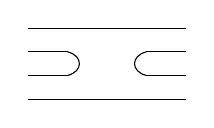
\begin{tikzpicture}
					\draw (0, 0) -- (2, 0);
					\draw (0, 0.3) -- (0.5, 0.3);
					\draw (0, 0.6) -- (0.5, 0.6);
					\draw (0.5, 0.3) .. controls (0.7, 0.35) and (0.7, 0.55) .. (0.5, 0.6);
					\draw (1.5, 0.3) -- (2, 0.3);
					\draw (1.5, 0.6) -- (2, 0.6);
					\draw (1.5, 0.3) .. controls (1.3, 0.35) and (1.3, 0.55) .. (1.5, 0.6);
					\draw (0, 0.9) -- (2, 0.9);
				\end{tikzpicture}
				\caption{Generator $U_2$ in TL$_4(\delta)$.}
				\label{fig:generator_temperley_lieb}
			\end{subfigure}
        	\end{figure}
        }
        
	\newdef{Frobenius algebra}{\index{Frobenius!algebra}
		An algebra $A$ equipped with a nondegenerate bilinear form $\eta:A\times A\rightarrow A$ satisfying the following condition for all $a,b,c\in A$:
		\begin{gather}
			\eta(ab,c)=\eta(a,bc)
		\end{gather}
	}

\subsection{Graded vector spaces}\label{section:graded_spaces}

	Similar to definition \ref{group:graded_ring} we can define the following:
	\newdef{Graded vector space}{\index{degree}\index{graded!vector space}
		Let $V_n$ be a vector space for all $n\in\mathbb{N}$. The vector space
		\begin{gather}
			\label{linalgebra:graded_vector_space}
			V = \bigoplus_{n\in\mathbb{N}} V_n
		\end{gather}
		is called a graded vector space. In fact one can replace $\mathbb{N}$ by any countable (finite or infinite) index set. For most operations however one requires the index set to be closed under addition operations. The index $n$ is often called the \textbf{degree} of the subspace $V_n$ in $V$.
	}
	
	\newdef{Graded algebra}{\index{graded!algebra}
		Let $V$ be a graded vector space with the additional structure of an algebra given by the multiplication $\star$. Then $V$ is a graded algebra if $\star$ maps $V^k\times V^l$ to $V^{k+l}$.
	}
	
	\newdef{Super vector space}{\index{super!vector space}
		A super vector space is defined as a $\mathbb{Z}_2$-graded vector space.
	}
	
	\begin{example}[Superalgebra]\index{super!algebra}\label{linalgebra:superalgebra}
		A $\mathbb{Z}_2$-graded algebra, i.e. there exists a decomposition
		\begin{gather}
			A = A_0\oplus A_1
		\end{gather}
		such that for all $i, j \mod 2$:
		\begin{gather}
			A_i\star A_j \subseteq A_{i+j}
		\end{gather}
	\end{example}
	
	\newdef{dg-algebra}{\index{dg-algebra}\label{linalgebra:dg_algebra}
		A differential graded algebra (often denoted by dg-algebra) is a graded algebra equipped with a differential of degree 1.
	}
	
	\newdef{Parity functor}{\index{parity}
		Consider the category $\mathbf{sVect}$ of super vector spaces. We can define the parity functor $\func{\Pi}{sVect}{sVect}$ as the functor which interchanges even and odd subspaces:
		\begin{align}
			(\Pi V)_0 &= V_1\\
			&\\
			(\Pi V)_1 &= V_0
		\end{align}
	}
	\newdef{Symmetric tensors}{
		Using the parity functor one can write the exterior algebra $\Lambda^\bullet(V)$ as the symmetric algebra $\text{Sym}^\bullet(\Pi V)$. In a similar way one can write the symmetric algebra on a super vector space $V=V_0\oplus V_1$ as $\text{Sym}^n(V)=\bigoplus_{p+q=n}\text{Sym}^p(V_0)\otimes\Lambda^q(V_1)$.
	}
        
\section[Linear maps]{Linear maps\footnote{Other names are \textbf{linear mapping} and \textbf{linear transformation}.}}
	
	\begin{property}
		Let $V$ be finite-dimensional $K$-vector space. Let $f:V\rightarrow V$ be a linear map. The following statements are equivalent:
        	\begin{itemize}
            		\item $f$ is injective
			\item $f$ is surjective
                	\item $f$ is bijective
		\end{itemize}
	\end{property}

	\newdef{Automorphism}{\index{automorphism}\label{linalgebra:automorphism}
		\nomenclature[S_Aut]{$\text{Aut}(V)$}{Set of automorphisms (invertible endomorphisms) on a set $V$.}
	    	An isomorphism from $V$ to $V$ is called an automorphism\footnote{In some case also called a \textbf{linear operator}, but this terminology is also used for a general linear map in operator theory (see chapter \ref{chapter:operator:algebras}).}. The set of all automorphisms  on $V$, which is in fact a group, is denoted by $\text{Aut}(V)$.
	}
    
	\newdef{General linear group\footnotemark}{\index{general linear group}
		\nomenclature[S_GL]{GL$(V)$}{General linear group: group of all automorphisms on a vector space $V$.}
		\footnotetext{This group is isomorphic to the general linear group of invertible matrices, hence the similar name and notation. (See definition \ref{linalgebra:GL_matrices})}
	    	The set of all automorphisms $f:V\rightarrow V$ is called the general linear group and denoted by GL$_K(V)$ or GL$(V)$ when the base field is clear.
	}

	\newdef{Rank}{\index{rank}\label{linalgebra:image_rank}
		The dimension of the image of a linear map is called the rank.
	}
	\newdef{Kernel}{\index{kernel}
	        The kernel of a linear map $f: V \rightarrow W$ is defined as the following subspace of $V$:
        	\begin{gather}
        		\text{ker}(f) = \{v\in V\ |\ f(v) = 0\}
	        \end{gather}
	}
	\newdef{Nullity}{\index{nullity}
		The dimension of the kernel is called the nullity.
	}
    
	\begin{theorem}
	    	A linear map $f:V\rightarrow W$ is injective if and only if $\text{ker}(f) = \{0\}$.
	\end{theorem}
	\begin{property}
	        Let $f:V\rightarrow W$ be a linear map. Let $U\leq V$. We have the following two properties of the restriction $f|_U$ of $f$ to $U$:
        	\begin{itemize}
			\item $\text{ker}\left(f|_U\right) = \text{ker}(f)\cap U$
        		\item $\text{im}\left(f|_U\right) \leq \text{im}(f)$
		\end{itemize}
	\end{property}
    
\subsection{Dimension}

        \begin{theorem}[Dimension theorem\footnotemark]\index{rank-nullity theorem}
		\footnotetext{Also called the \textbf{rank-nullity theorem}.}
		Let $f: V \rightarrow W$ be a linear map.
	        \begin{gather}
	                \label{linalgebra:dimension_theorem}
	                \dim(\text{\upshape im}(f)) + \dim(\text{\upshape ker}(f)) = \dim(\text{\upshape V})
	        \end{gather}
        \end{theorem}

        \begin{property}
		Two $K$-vector spaces are isomorphic if and only if they have the same dimension.
	\end{property}
    
\subsection{Homomorphisms}

	\newdef{Homomorphism space}{\index{morphism!of vector spaces}
		\nomenclature[S_Hom]{$\hom(V, W)$}{Set of morphisms from a set $V$ to a set $W$.}
    		Let $V,W$ be two K-vector spaces. The set of all linear maps between $V$ and $W$ is called the homomorphism space of $V$ to $W$, or shorter: the 'hom-space' of $V$ to $W$.
	    	\begin{equation}
        		\label{linalgebra:hom_space}
        		\hom_K(V, W) = \{f:V\rightarrow W\ |\ \text{f is linear}\}
		\end{equation}
	}
	\begin{theorem}\label{linalgebra:hom_dimension}
	    	If $\ V,W$ are two finite-dimensional K-vector spaces we have:
        	\begin{equation}
        		\dim\left(\emph{Hom}_K(V,W)\right) =\dim(V)\cdot\dim(W)
		\end{equation}
	\end{theorem}
        
	\newdef{Endomorphism ring}{
		\nomenclature[S_End]{$\text{End}(V)$}{Ring of endomorphisms on a set $V$.}
		The space $\hom_K(V, V)$ with the composition as multiplication forms a ring, the endomorphism ring. It is denoted by $\text{End}_K(V)$ or $\text{End}(V)$.
	}
	\begin{property}
		The endomormphism ring $\text{End}(V)$ forms a Lie algebra\footnote{See also \ref{lie:end_as_lie_algebra}.} when equipped with the commutator $[A, B] = A\circ B - B\circ A$.
	\end{property}
	
	\begin{property}[Jordan-Chevalley decomposition]\index{Jordan!decomposition}\index{semisimple!operator}\index{nilpotent}\label{linalgebra:jordan_chevalley}
		Every endomorphism $A$ can be decomposed as follows:
		\begin{equation}
			A = A_{ss} + A_n
		\end{equation}
		where
		\begin{itemize}
			\item $A_{ss}$ is \textbf{semisimple}, i.e. for every the invariant subspace of $A_{ss}$ there exists an invariant complementary subspace.
			\item $A_n$ is \textbf{nilpotent}, i.e. $\exists k\in\mathbb{N}: A_n^k = 0$.
		\end{itemize}
		Furthermore, this decomposition is unique and the endomorphisms $A_{ss}, A_n$ can be written as polynomials in $A$.
	\end{property}
    
	\newdef{Minimal polynomial}{\index{minimal polynomial}
	    	Let $f\in\text{End}(V)$ and $V$ a finite-dimensional K-vector space. The monic polynomial $\mu_f(x)$ of the lowest order such that $\mu_f(f)=0$ is called the minimal polynomial of $f$.
	}
	\begin{property}\label{linalgebra:minimal_polynomial_divisor}
		Let $f\in\text{End}(V)$. Let $\mu_f(x)$ be the minimal polynomial of $f$. Let $\varphi(x)\in K[x]$. If $\varphi(f) = 0$, then the minimal polynomial $\mu_f(x)$ divides $\varphi(x)$. 
	\end{property}
    
\subsection{Dual space}

	\newdef{Dual space}{\index{dual!space}
	    	Let $V$ be a K-vector space. The dual space $V^*$ of $V$ is the following vector space:
	    	\begin{equation}
			\label{linalgebra:dual_space}
		        V^*:=\text{Hom}_K(V, K)=\{f:V\rightarrow K\ :\ f\text{ is a linear map}\}
		\end{equation}
	}
	\newdef{Linear form}{\index{linear!form}
	    	The elements of $V^*$ are called \textit{linear forms}.
	}
	\begin{property}\label{linalgebra:dual_space_dimension}
		From theorem \ref{linalgebra:hom_dimension} it follows that $\dim(V^*) = \dim(V)$.
	\end{property}
	\begin{remark}
		If $V$ is infinite-dimensional, theorem \ref{linalgebra:dual_space_dimension} is not valid. In the infinite-dimensional case we \textbf{always} have $|V^*|>|V|$ (where we now use the cardinality instead of the dimension).
	\end{remark}
    
	\newdef{Dual basis}{
    		Let $\mathcal{B} = \{e_1, e_2, ..., e_n\}$ be a basis for a finite-dimensional K-vector space $V$. We can define a basis $\mathcal{B}^* = \{\varepsilon_1, \varepsilon_2, ..., \varepsilon_n\}$ for $V^*$, called the dual basis of $\mathcal{B}$, as follows:
    		\begin{equation}
			\label{linalgebra:dual_basis}
        		\boxed{\varepsilon_i:V\rightarrow K:\sum_{j=1}^na_ie_i\mapsto a_i}
		\end{equation}
		The relation between the basis and dual basis can also be written as:
		\begin{equation}
			\label{linalgebra:dual_basis_2}
			\varepsilon^i(e_j) = \delta^i_j
		\end{equation}
	}
    
	\newdef{Dual map}{\index{dual!map}\label{linalgebra:transpose}
		Let $f:V\rightarrow W$ be a linear map. The linear map $f^*:W^*\rightarrow V^*:\varphi\rightarrow\varphi\circ f$ is called the dual map or \textbf{transpose} of $f$.
	}
	\newnot{Transpose}{\index{transpose}
		When $V=W$ the dual map $f^*$ is often denoted by $f^T$.
	}
    
    \newdef{Natural pairing}{\index{natural!pairing}
    	The natural pairing of $V$ and its dual $V^*$ is defined as the following bilinear map:
        \begin{equation}
        	\label{linalgebra:natural_pairing}
            \langle v, v^*\rangle = v^*(v)
        \end{equation}
    }

\subsection{Convex functions}
	
	\newdef{Convex function}{\index{convex!function}
		Let $X$ be a convex subset of $V$. A function $f:X\rightarrow \mathbb{R}$ is convex if for all $x, y\in X$ and $t\in[0, 1]$:
		\begin{equation}
			f(tx + (1-t)y) \leq tf(x) + (1-t)f(y)
		\end{equation}
	}
	\begin{remark}
		For a concave function we have to turn the inequality around.
	\end{remark}
	\begin{result}
		A linear map $f:X\rightarrow\mathbb{R}$ is both convex and concave.
	\end{result}
	
	\begin{theorem}[Karamata's inequality]\index{Karamata's inequality}
		Let $I\subset\mathbb{R}$ be an interval and let $f:I\rightarrow\mathbb{R}$ be a convex function. If $(x_1, ..., x_n)$ is a tuple that majorizes $(y_1, ..., y_n)$, i.e. $\forall k\leq n$
		\begin{align}
			\sum_{i=1}^nx_i &= \sum_{i=1}^ny_i\\
			x_{(1)} + ... + x_{(k)}&\geq y_{(1)} + ... + y_{(k)}
		\end{align}
		where $x_{(i)}$ denotes the ordering\footnote{In decreasing order: $x_{(1)}\geq...\geq x_{(n)}$.} of the tuple $(x_1, ..., x_n)$. Then
		\begin{equation}
			\sum_{i=1}^nf(x_i)\geq \sum_{i=1}^nf(y_i)
		\end{equation}
	\end{theorem}

\section{Inner product}\label{linalgebra:innerproduct}

    In this section all vector spaces $V$ will be defined over $\mathbb{R}$ or $\mathbb{C}$.

\subsection{Inner product space}

    \newdef{Inner product}{\index{inner!product}
        A map $\langle\cdot|\cdot\rangle:V\times V\rightarrow\mathbb{C}$ is called an inner product on $V$ if it satisfies the following properties for all $v,w\in V$ and $\lambda\in\mathbb{C}$:
        \begin{enumerate}
            \item \textbf{Conjugate symmetry}: $\langle v|w \rangle = \langle w|v \rangle^*$,
            \item \textbf{Linearity in the first argument}: $\langle \lambda u+v|w \rangle = \lambda\langle u|w \rangle + \langle v|w \rangle$,
            \item \textbf{Nondegeneracy}: $\langle v|v \rangle = 0 \iff v = 0$, and
            \item \textbf{Positive-definiteness}: $\langle v|v \rangle \geq 0$.
        \end{enumerate}
    }
    \begin{remark}\index{Hermitian!form}\label{linalgebra:NDH_form}
        Inner products are special cases of \textbf{nondegenerate Hermitian forms} which do not satisfy the positive-definiteness property (these often occur when working over $\mathbb{C}$).
    \end{remark}

    \begin{result}\index{sesquilinear}
        The first two properties have the result of conjugate linearity in the second argument:
        \begin{gather}
            \langle f|\lambda g + \mu h \rangle = \overline{\lambda}\langle f|g \rangle + \overline{\mu}\langle f|h \rangle
        \end{gather}
        Therefore these two properties together are often combined into a \textbf{sesquilinearity} property. When the underlying field is restricted to $\mathbb{R}$, such that the conjugate symmetry property is replaced by symmetry, the inner product becomes a bilinear form.
    \end{result}

    \newdef{Inner product space\footnotemark}{
        \footnotetext{Sometimes called a \textbf{pre-Hilbert space}.}
        A vector space equipped with an inner product $\langle\cdot|\cdot\rangle$.
    }

    \newdef{Metric dual\footnotemark}{
        \footnotetext{See also Definition \ref{riemann:flat_map}.}
        Using the inner product (or any other nondegenerate Hermitian form) one can define the metric dual of a vector $v$ by the following map:
        \begin{gather}
            \label{linalgebra:metric_dual}
            L:V\rightarrow V^*:v\mapsto \langle v|\cdot \rangle.
        \end{gather}
    }
    \newdef{Adjoint operator}{\index{adjoint}\index{Hermitian}\index{self-adjoint}\label{linalgebra:adjoint_operator}
        Let $A$ be a linear operator on $V$. The (\textbf{Hermitian}) adjoint of $A$ is defined as the linear operator $A^\dag$ that satisfies
        \begin{gather}
            \langle A^\dag v|w\rangle = \langle v|Aw\rangle
        \end{gather}
        for all $v,w\in V$. Alternatively, one can define the adjoint using the transpose and metric dual as follows:
        \begin{gather}
            A^\dag = L^{-1} \circ A^T \circ L.
        \end{gather}
        If $A=A^\dag$, then A is said to be \textbf{Hermitian} or \textbf{self-adjoint}. (In Chapter \ref{chapter:normed_spaces} a distinction will be made between these two notions.)
    }
    \begin{result}
        The Hermitian adjoint of a complex matrix $A\in\mathbb{C}^{m\times n}$ is given by
        \begin{gather}
            A^\dag = \overline{A}^T,
        \end{gather}
        where $\overline{A}$ denotes the complex conjugate of $A$ and $A^T$ the transpose of $A$.
    \end{result}

\subsection{Orthogonality}\label{linalgebra:section:orthogonality}

    \newdef{Orthogonal}{\index{orthogonal}\label{linalgebra:orthogonal}
        Consider two vectors $v,w\in V$ in an inner product space. These vectors are said to be orthogonal, denoted by $v\perp w$,  if they obey the following relation:
        \begin{gather}
            \langle v|w \rangle = 0.
        \end{gather}
        An \textbf{orthogonal system} is a collection of vectors, none of them equal to 0, that are mutually orthogonal.
    }
    \begin{property}
        Orthogonal systems are linearly independent.
    \end{property}

    \newdef{Orthonormal}{\index{orthonormal}\label{linalgebra:orthonormal}
        A collection of vectors $S$ is said to be orthonormal if it forms an orthogonal system and if all the elements $v\in S$ obey the following relation:
        \begin{gather}
            \langle v|v \rangle = 1.
        \end{gather}
    }
    \newdef{Orthogonal complement}{\index{complement}\label{linalgebra:orthogonal_complement}
        Let $W$ be a subspace of an inner product space $V$. The orthogonal complement of $W$ is defined as the following subspace:
        \begin{gather}
            W^\perp := \{v\in V\mid\forall w\in W:\langle v|w\rangle = 0\}.
        \end{gather}
    }
    \sremark{$W^\perp$ is pronounced as 'W-perp'.}

    \begin{property}[Complements]
        Let $V$ be a finite-dimensional inner product space. The orthogonal complement $W^\perp$ is a complementary subspace to $W$, i.e. $W\oplus W^\perp=V$.
    \end{property}
    \begin{result}\label{linalgebra:perp_of_perp}
        Let $W\leq V$ where $V$ is a finite-dimensional inner product vector space. Taking orthogonal complements defines an involution:
        \begin{gather}
            (W^\perp)^\perp = W.
        \end{gather}
    \end{result}

    \newdef{Orthogonal projection}{\index{projection}\label{linalgebra:orthogonal_projection}
        Let $V$ be a finite-dimensional inner product vector space and consider a subspace $W\leq V$. Consider a vector $w\in W$ and let $\{w_1, \ldots, w_k\}$ be an orthonormal basis of $W$. The projections of $v\in V$ on $W$ and $w\in W$ are defined as follows:
        \begin{align}
            \text{proj}_W(v) &:= \sum_{i=1}^k\langle v|w_i \rangle w_i\\
            \text{proj}_w(v) &:= \stylefrac{\langle v|w \rangle}{\langle w|w \rangle}w.
        \end{align}
    }
    \begin{property}
        Orthogonal projections satisfy the following conditions:
        \begin{itemize}
            \item $\forall w\in W:\text{proj}_W(w) = w$, and
            \item $\forall u\in W^\perp:\text{proj}_W(u) = 0$.
        \end{itemize}
    \end{property}

    \newmethod{Gram-Schmidt orthonormalization}{\label{linalgebra:inner_product:gram_schmidt}
        Let $\{u_i\}_{i\leq n}$ be a set of linearly independent vectors. An orthonormal set $\{e_i\}_{i\leq n}$ can be constructed out of $\{u_i\}_{i\leq n}$ using the following procedure:
        \begin{enumerate}
            \item Orthogonalization:
                \begin{gather}
                    \begin{aligned}
                        w_1& = u_1&\\
                        w_2& = u_2 - \stylefrac{\langle u_2|w_1\rangle}{||u_2||^2}w_1&\\
                        &\vdots&\\
                        w_n& = u_n - \sum_{i=1}^{n-1}\stylefrac{\langle u_n|w_i\rangle}{||u_n||^2}w_i&
                    \end{aligned}
                \end{gather}
            \item Normalization:
                \begin{gather}
                    \begin{aligned}
                        e_1& = \stylefrac{w_1}{||w_1||}&\\
                        e_2& = \stylefrac{w_2}{||w_2||}&\\
                        &\vdots&\\
                        e_n& = \stylefrac{w_n}{||w_n||}&
                    \end{aligned}
                \end{gather}
        \end{enumerate}
    }

    \newdef{Householder transformation}{\index{Householder transformation}\label{linalgebra:householder_transformation}
        Let $v$ be an element of an inner product space $V$. The Householder transformation generated by $v$ is given by the linear map
        \begin{gather}
            \sigma_v:V\rightarrow V:w\mapsto w - 2\frac{\langle w|v \rangle}{\langle v|v \rangle}v.
        \end{gather}
        This transformation amounts to a reflection in the hyperplane orthogonal to $v$.
    }

    \newdef{Angle}{\index{angle}\label{linalgebra:angle}
        Let $v,w$ be elements of an inner product space $V$. The angle $\theta$ between $v$ and $w$ is defined by the following formula:
        \begin{gather}
            \cos\theta := \stylefrac{\langle v|w \rangle}{||v||||w||}.
        \end{gather}
    }
\section{Matrices}
	
	\begin{notation}\label{linalgebra:matrix_set}
	        The set of all $m\times n$-matrices defined over the field $K$ is denoted by $M_{m,n}(K)$. If $m=n$, the set is denoted by $M_n(K)$.
	\end{notation}
	
	\begin{property}[Dimension]\index{dimension}\label{linalgebra:dimension_of_matrix_space}
		The dimension of $M_{m,n}(K)$ as a vector space is $mn$.
	\end{property}
    
	\newdef{Trace}{\index{trace}\label{linalgebra:trace}
	        Let $A = (a_{ij})\in M_n(K)$. We define the trace of $A$ as follows:
    		\begin{gather}
			\text{tr}(A) = \sum_{i=1}^na_{ii}
		\end{gather}
	}
	\begin{property}\label{linalgebra:trace_commutative}
		Let $A, B\in M_n(K)$. The trace satisfies the following properties:
	        \begin{enumerate}
        		\item $\text{tr}:M_n(K)\rightarrow K$ is a linear map
			\item $\text{tr}(AB) = \text{tr}(BA)$
			\item $\text{tr}(AB) \neq \text{tr}(A)\text{tr}(B)$
        		\item $\text{tr}(A^T) = \text{tr}(A)$
		\end{enumerate}
	\end{property}
    
	\newformula{Hilbert-Schmidt norm\footnotemark}{\index{Frobenius!norm}\index{Hilbert-Schmidt norm}
    		\footnotetext{Also called the \textbf{Frobenius norm}.}
    		The Hilbert-Schmidt norm is given by the following formula:
	        \begin{gather}
        		\label{linalgebra:hilbert_schmidt_norm}
        		||A||^2_{HS} = \sum_{i, j}|A_{ij}|^2 = \text{tr}(A^\dag A)
	        \end{gather}
        	If one identifies $M_{n}(\mathbb{C})$ with $\mathbb{C}^{2n}$ then this norm equals the standard Hermitian norm.
	}

	\newformula{Hadamard product}{\index{Hadamard!product}
    		The Hadamard product of two matrices $A, B\in M_{m\times n}(K)$ is defined as the entry-wise product:
        	\begin{gather}
        		(A\circ B)_{ij} = A_{ij}B_{ij}
        	\end{gather}
	}
    
	\newdef{General linear group}{\index{general linear group}\label{linalgebra:GL_matrices}
		\nomenclature[S_GLn]{GL$(n,K)$}{General linear group: group of all invertible $n$-dimensional matrices over the field $K$.}
	        The set of invertible matrices is called the general linear group and is denoted by GL$_n(K)$ or GL$(n, K)$.
	}
	\begin{property}
		For all $A\in\text{GL}_n(K)$ we have:
	        \begin{itemize}
			\item $A^T\in\text{GL}_n(K)$
		        \item $\left(A^T\right)^{-1}=\left(A^{-1}\right)^T$
		\end{itemize}
	\end{property}
    
	\begin{property}\label{linalgebra:dim_columns_rows}
		Let $A\in M_{m,n}(K)$. Denote the set of columns as $\{A_1, A_2, ..., A_n\}$ and the set of rows as $\{R_1, R_2, ..., R_m\}$. The set of columns is a subset of $K^m$ and the set of rows is a subset of $K^n$ and as such we can define their span. These spaces satisfy the following property:
		\begin{gather}
			\dim(\text{span}(A_1, ..., A_n)) = \dim(\text{span}(R_1, ..., R_m))
		\end{gather}
	\end{property}
	
	\newdef{Rank}{\index{rank}
		Using the invariance relation from previous property we can define the rank of a matrix $A\in M_{m,n}(K)$ as follows:
		\begin{gather}
			\label{linalgebra:matrix_rank}
        		\text{rk}(A) := \dim(\text{span}(A_1, ..., A_n)) \overset{\ref{linalgebra:dim_columns_rows}}{=} \dim(\text{span}(R_1, ..., R_m))
		\end{gather}
	}
    
	\begin{property}\label{linalgebra:rank_properties}
	        The rank of a matrix has the following properties:
        	\begin{enumerate}
			\item $\text{rk}(AC)\leq\text{rk}(A)$ and $\text{rk}(AC)\leq\text{rk}(C)$
        		\item $\text{rk}(BC)=\text{rk}(C)$
		        \item $\text{rk}(BD)=\text{rk}(D)$
		\end{enumerate}
		where $A\in M_{m,n}(K)$, $B\in\text{GL}_n(K)$, $C\in M_{n,r}(K)$ and $D\in M_{r,n}(K)$.
	\end{property}
	\begin{property}\label{linalgebra:dim_matrix_left_multiplication}
	        Let $A\in M_{m,n}(K)$. We first define the following linear map:
        	\begin{gather}
			\label{linalgebra:matrix_left_multiplication}
        		L_A:K^n\rightarrow K^m:v\mapsto Av
		\end{gather}
	        This map has the following properties:
        	\begin{enumerate}
        		\item $\text{im}(L_A) = \text{span}(A_1, ..., A_n)$
			\item $\dim(\text{im}(L_A))=\text{rk}(A)$
		\end{enumerate}
	\end{property}
	\sremark{The second property is a direct consequence of the first one together with definition \ref{linalgebra:matrix_rank}.}
    
\subsection{System of equations}

	\begin{property}\label{linalgebra:matrix_and_equations}
	        Let $AX=w$ with $A\in M_{m,n}(K)$, $w\in K^m$ and $X\in K^n$ be a system of $m$ equations in $n$ variables. Let $L_A$ be the linear map as defined in equation \ref{linalgebra:matrix_left_multiplication}. We then have the following properties:
        	\begin{enumerate}
			\item The system is false if and only if $w\not\in\text{im}(L_A)$.
        		\item If the system is not false, the solution set is an affine space. If $v_0\in K^n$ is a solution, then the solution set is given by: $L_A^{-1}(w)=v_0+\text{ker}(L_A)$.
		        \item If the system is homogeneous ($AX=0$), then the solution set is equal to $\text{ker}(L_A)$.
		\end{enumerate}
	\end{property}
	\begin{property}[Uniqueness]\label{linalgebra:rank_unique_solution}
	        Let $AX=w$ with $A\in M_n(K)$ be a system of $n$ equations in $n$ variables. If $\text{rk}(A)=n$, then the system has a unique solution.
	\end{property}
	
	\newformula{Cramer's rule}{\index{Cramer}
    		Let $AX = w$ be a system of linear equations where the matrix $A$ has a nonzero determinant. Then Cramer's rule gives a unique solution where the unknowns are given by;
		\begin{gather}
			\label{linalgebra:cramers_rule}
			X_i = \stylefrac{\det(A_i)}{\det(A)}
		\end{gather}
		where $A_i$ is the matrix obtained by replacing the $i^{th}$ column of $A$ by the column matrix $w$.
	}
    
\subsection{Coordinates and matrix representations}

        \newdef{Coordinate vector}{\label{linalgebra:coordinate_vector}
        	Let $\mathcal{B} = \{b_1, ..., b_n\}$ be a basis of $V$. Let $v\in V$ such that $v=\sum_{i=1}^n\lambda_ib_i$. We define the coordinate vector of $v$ with respect to $\mathcal{B}$ as $(\lambda_1, ..., \lambda_n)^T$. The $\lambda_i$'s are called the \textbf{coordinates} of $v$ with respect to $\mathcal{B}$.
        }
        \newdef{Coordinate isomorphism}{\label{linalgebra:coordinate_isomorphism}
        	With the previous definition in mind we can define the coordinate isomorphism of $v$ with respect to $\mathcal{B}$ as follows:
        	\begin{gather}
			\boxed{\beta:V\rightarrow K^n:\sum_{i=1}^n\lambda_ib_i\mapsto(\lambda_1, ..., \lambda_n)^T}
		\end{gather}
        }
        
        \newdef{Matrix representation}{\label{linalgebra:matrix_representation}
        	Let $V$ be an $n$-dimensional K-vector space and $W$ an $m$-dimensional K-vector space. Let $f:V\rightarrow W$ be a linear map. Let $\mathcal{B}=\{b_1, ..., b_n\}, \mathcal{C} = \{c_1, ..., c_m\}$ be a basis for $V$, respectively $W$. The matrix representation of $f$ with respect to $\mathcal{B}$ and $\mathcal{C}$ can be derived as follows: For every $j\in\{1, ..., n\}$ we can write $f(b_j) = \sum_{i=1}^ma_{ij}c_i$, so with this in mind we can define the matrix $(a_{ij})\in M_{m,n}(K)$ as the matrix represenation of $f$.
        }
        \newnot{Matrix representation of a linear map}{
        	The matrix representation of $f$ with respect to $\mathcal{B}$ and $\mathcal{C}$ is denoted by $A_{f, \mathcal{B}, \mathcal{C}}$.
        }
        
        \newmethod{Construction of a matrix representation}{\label{linalgebra:method:matrix_representation}
        	From definition \ref{linalgebra:matrix_representation} we can see that $j$-th column of $A_{f, \mathcal{B}, \mathcal{C}}$ coincides with the coordinate vector of $f(b_j)$ with respect to $\mathcal{C}$. We use this relation to construct $A_{f, \mathcal{B}, \mathcal{C}}$ by writing for every $j\in\{1, ..., n\}$ the coordinate vector of $f(b_j)$ in the $j$-th column.
        }
        
        \begin{theorem}\label{linalgebra:theorem:matrix_representation}
		Let $(\lambda_1, ..., \lambda_n)^T$ be the coordinate vector of $v\in V$ with respect to $\mathcal{B}$. Let $(\mu_1, ..., \mu_m)^T$ be the coordinate vector of $f(v)$ with respect to $\mathcal{C}$. Then the following relation holds:
            	\begin{gather}
			\left(
			\begin{array}{c}
				\mu_1\\
				\vdots\\
				\mu_m
			\end{array}\right)
	                = A_{f, \mathcal{B}, \mathcal{C}}
        	        \left(\begin{array}{c}
				\lambda_1\\
				\vdots\\
				\lambda_n
			\end{array}\right)
		\end{gather}
	\end{theorem}
        
        \begin{theorem}\label{linalgebra:theorem:map_matrix_link}
		For every matrix $A\in M_{m,n}(K)$ there exists a linear map $f:V\rightarrow W$ such that $A_{f, \mathcal{B}, \mathcal{C}} = A$.
	\end{theorem}
        On the other hand we also have the following theorem:
        \begin{theorem}
		Let $f:K^n\rightarrow K^m$ be a linear map. There exists a matrix $A\in M_{m,n}(K)$ such that $f=L_A$.
	\end{theorem}
        \begin{theorem}
		Let $\beta$ and $\gamma$ be the coordinate isomorphisms with respect to respectively $\mathcal{B}$ and $\mathcal{C}$. From theorem \ref{linalgebra:theorem:matrix_representation} it follows that:
        	\begin{gather}
			\gamma(f(v)) = A_f\cdot\beta(v)
		\end{gather}
        	or alternatively
        	\begin{gather}
			\gamma\circ f = L_{A_f}\circ\beta
		\end{gather}
	\end{theorem}
        
        \begin{theorem}\label{linalgebra:theorem:matrix_composition_hom}
	        The map $\text{Hom}_K(V,W)\rightarrow M_{m,n}(K):f\mapsto A_f$ is an isomorphism and for every $f\in\text{Hom}_K(V,W)$ and $g\in \text{Hom}_K(W,U)$ we have:
		\begin{gather}
			A_{g\circ f} = A_gA_f
		\end{gather}
	\end{theorem}
	
	\begin{theorem}\label{linalgebra:theorem:matrix_composition_end}
	        The map $\text{End}_K(V)\rightarrow M_n(K):f\mapsto A_{f, \mathcal{B}, \mathcal{B}}$ is an isomorphism and for every $f,g\in\text{End}_K(V)$ we have:
        	\begin{gather}
			A_{g\circ f} = A_gA_f
		\end{gather}
	\end{theorem}
	
        \begin{theorem}\label{linalgebra:matrix_invertable_map}
	        Let $f\in\text{End}_K(V)$. Let $A_f$ be the corresponding matrix representation. The linear map $f$ is invertible if and only if $A_f$ is invertible. Furthermore, if $A_f$ is invertible, we have that \[\left(A_f\right)^{-1} = A_{f^{-1}}\] In other words, the following map is an isomorphism\footnotemark:
	        \begin{gather}
	        	\text{GL}_K(V)\rightarrow\text{GL}_n(K):f\mapsto A_f
	        \end{gather}
	        \footnotetext{Follows from theorem \ref{linalgebra:theorem:matrix_composition_end}.}
	\end{theorem}
        \remark{The sets GL$_K(V)$ and GL$_N(K)$ are groups. So the previous theorem states that the map $f\mapsto A_f$ is a group isomorphism.}
        
        \begin{theorem}
		Let $V = K^n$. Let $f\in V^*$. From construction \ref{linalgebra:method:matrix_representation} it follows that $A_f = (f(e_1), ..., f(e_n))\in M_{1,n}(K)$ with respect to the standard basis of $V$. This combined with theorem \ref{linalgebra:theorem:matrix_representation} gives:
	        \begin{gather}
			f(\lambda_1, ..., \lambda_n)^T = (f(e_1), ..., f(e_n))(\lambda_1, ..., \lambda_n)^T = \sum_{i=1}^nf(e_i)\lambda_i
		\end{gather}
        	or alternatively with $\{\varepsilon_1, ..., \varepsilon_n\}$ the dual basis to the standard basis of $V$:
	        \begin{gather}
        	    	\label{linalgebra:map_in_function_of_dual_basis}
			\boxed{f = \sum_{i=1}^nf(e_i)\varepsilon_i}
		\end{gather}
	\end{theorem}
        
        \begin{theorem}
		Let $f:V\rightarrow W$ be a linear map. Let $f^*:W^*\rightarrow V^*$ be the corresponding dual map. If $A_f$ is the matrix representation of $f$ with respect to $\mathcal{B}$ and $\mathcal{C}$, then the transpose $A_f^T$ is the matrix representation of $f^*$ with respect to the dual basis of $\mathcal{C}$ and the dual basis of $\mathcal{B}$.
	\end{theorem}
        
\subsection{Coordinate transforms}
        
        \newdef{Transition matrix}{\label{linalgebra:transition_matrix}
        	Let $\mathcal{B} = \{b_1, ..., b_n\}$ and $\mathcal{B}' = \{b_1', ..., b_n'\}$ be two bases of $V$. Every element of $\mathcal{B}'$ can be written as a linear combination of elements in $\mathcal{B}$:
        	\begin{gather}
        		b_j' = q_{1j}b_1 + ... + q_{nj}b_n
        	\end{gather}
	        The matrix $Q = (q_{ij})\in M_n(K)$ is called the transition matrix from the 'old' basis $\mathcal{B}$ to the 'new' basis $\mathcal{B}'$.}
        
        \begin{theorem}\label{linalgebra:theorem:transition_matrix}
		Let $\mathcal{B}, \mathcal{B}'$ be two basis of $V$. Let $Q$ be the transition matrix from $\mathcal{B}$ to $\mathcal{B}'$. We find the following statements:
	        \begin{enumerate}
			\item Let $\mathcal{C}$ be an arbitrary basis of $V$ with $\gamma$ the corresponding coordinate isomorphism. Define the following matrices:
        	        	\[
        	        		B=(\gamma(b_1), ..., \gamma(b_n))\quad\text{and}\quad B'=(\gamma(b_1'), ..., \gamma(b_n'))
        	        	\]
		                Then $BQ = B'$.
			\item $Q\in\text{GL}_n(K)$ and $Q^{-1}$ is the transition matrix from $\mathcal{B}'$ to $\mathcal{B}$.
                	\item Let $v\in V$ with $(\lambda_1, ..., \lambda_n)^T$ the coordinate vector with respect to $\mathcal{B}$ and $(\lambda_1', ..., \lambda_n')^T$ the coordinate vector with respect to $\mathcal{B}'$. Then:
                	\[
		                Q\left(
				\begin{array}{c}
					\lambda_1'\\
                			\vdots\\
			        	\lambda_n'
				\end{array}
                        	\right)
                        	=
		                \left(
                		\begin{array}{c}
					\lambda_1\\
                			\vdots\\
			        	\lambda_n
				\end{array}
                        	\right)
				\quad\text{and}\quad
                        	\left(
                        	\begin{array}{c}
					\lambda_1'\\
                        		\vdots\\
			        	\lambda_n'
				\end{array}
		                \right)
                	        =
                	        Q^{-1}\left(
                	        \begin{array}{c}
					\lambda_1\\
                		        \vdots\\
			                \lambda_n
				\end{array}
                        	\right)
			\]
		\end{enumerate}
	\end{theorem}
        
	\begin{theorem}\label{linalgebra:theorem:transition_matrix_representation}
        	Let $V,W$ be two finite-dimensional K-vector spaces. Let $\mathcal{B}, \mathcal{B}'$ be two bases of $V$ and $\mathcal{C}, \mathcal{C}'$ two bases of $W$. Let $Q, P$ be the transition matrices from $\mathcal{B}$ to $\mathcal{B}'$ and from $\mathcal{C}$ to $\mathcal{C}'$ respectively. Let $A=A_{f, \mathcal{B}, \mathcal{C}}$ and $A' = A_{f, \mathcal{B}', \mathcal{C}'}$. Then:
	        \begin{gather}
        	    	A' = P^{-1}AQ
        	\end{gather}
	\end{theorem}
        \begin{result}
		Let $f\in \text{End}_K(V)$ and let $Q$ be the transition matrix. From theorem \ref{linalgebra:theorem:transition_matrix_representation} it follows that:
            	\begin{gather}
	            	A'=Q^{-1}AQ
        	\end{gather}
	\end{result}

        \newdef{Matrix conjugation}{\index{conjugacy class}\index{matrix!conjugation}\label{linalgebra:conjugacy_class}
        	Let $A\in M_n(K)$. The set
        	\begin{gather}
	            	\{Q^{-1}AQ\ |\ Q\in\text{GL}_n(K)\}
        	\end{gather}
	        is called the conjugacy class\footnotemark\ of $A$. Another name for conjugation is \textbf{similarity transformation}.
        	\footnotetext{This is the general definition of conjugacy classes for groups. Furthermore, these classes induce a partitioning of the group.}
	}
        \begin{remark}
        	If $A$ is a matrix representation of a linear operator $f$, then the conjugacy class of $A$ consists out of every possible matrix representation of $f$.
        \end{remark}
        
        \begin{property}
        	From property \ref{linalgebra:trace_commutative} it follows that the trace of a matrix is invariant under similarity transformations:
        	\begin{gather}
            		\label{linalgebra:trace_invariance}
            		\boxed{\text{tr}(Q^{-1}AQ) = \text{tr}(A)}
	        \end{gather}
        \end{property}
        
        \newdef{Matrix congruence}{\index{matrix!congruence}\label{linalgebra:matrix_congruence}
        	Let $A, B\in M_n(K)$. If there exists a matrix $P$ such that
	        \begin{gather}
        	    	A = P^TBP
        	\end{gather}
	        then the matrices are said to be congruent.
        }
        \begin{property}
        	Every matrix congruent to a symmetric matrix is also symmetric.
        \end{property}
        
        \begin{theorem}\label{linalgebra:theorem:orthogonal_transition_matrix}
        	Let $(V, \langle .|. \rangle)$ be an inner-product space defined over $\mathbb{R}$ (or $\mathbb{C}$). Let $\mathcal{B}, \mathcal{B}'$ be two orthonormal bases of $V$ and let $Q$ be the transition matrix. Then $Q$ is orthogonal:
        	\begin{gather}
	        	Q^TQ = \mathbbm{1}_n
	        \end{gather}
	\end{theorem}

\subsection{Determinant}

    	\newdef{Minor}{
        	The $(i, j)$-th minor of $A$ is defined as:\[\det(A_{ij})\] where $A_{ij}\in M_{n-1}(K)$ is the matrix obtained by removing the $i$-th row and the $j$-th column from $A$.
	}
        \newdef{Cofactor}{
        	The cofactor $\alpha_{ij}$ of the matrix element $a_{ij}$ is equal to:\[(-1)^{i+j}\det(A_{ij})\]where $\det(A_{ij})$ is the minor as previously defined.
	}
        \newdef{Adjugate matrix}{\label{linalgebra:adjugate_matrix}
	        The adjugate matrix of $A\in M_n(K)$ is defined as follows:
	       	\begin{gather}
	            	\text{adj}(A) := \left(
	                \begin{array}{cccc}
				\alpha_{11}&\alpha_{21}&\dotsm&\alpha_{n1}\\
		                \alpha_{12}&\alpha_{22}&\dotsm&\alpha_{n2}\\
		                \vdots&\vdots&\vdots&\vdots\\
		                \alpha_{1n}&\alpha_{2n}&\dotsm&\alpha_{nn}\\
			\end{array}
        	        \right)
		\end{gather}
        	or shorter: $\text{adj}(A) = (\alpha_{ij})^T$.
        }
        \begin{remark*}
		It is important to notice that we have to transpose the matrix after the elements have been replaced by their cofactor.
	\end{remark*}
        
        \begin{property}\label{linalgebra:determinant_properties}
	        Let $A,B\in M_n(K)$. Denote the columns of $A$ as $A_1, \dotso, A_n$. We have the following properties of the determinant:
	        \begin{enumerate}
			\item $\det(A^T) = \det(A)$
	                \item $\det(AB) = \det(BA) = \det(A)\det(B)$
	                \item $\det(A_1, \dotso, A_i+\lambda A_i', \dotso, A_n) = \det(A_1, \dotso, A_i, \dotso, A_n) + \lambda\det(A_1, \dotso,A_i', \dotso, A_n)$ for all $A_i,A_i'\in M_{n,1}(K)$.
	                \item If two columns of $A$ are equal then $\det(A) = 0$.
	                \item $\det(A_{\sigma(1)},\dotso,A_{\sigma(n)}) = \text{sgn}(\sigma)\det(A_1,\dotso,A_n)$
	                \item The determinant can be evaluated as follows:
	                	\begin{gather}
					\det(A) = \sum_{i=1}^n(-1)^{i+k}a_{ik}\det(A_{ik})
				\end{gather}
		\end{enumerate}
		\end{property}
        
	\begin{theorem}\label{linalgebra:theorem:rank_det_equivalence}
        	Let $A\in M_n(K)$, the following statements are equivalent:
        	\begin{enumerate}
			\item $\det(A) \neq 0$
        	        \item $\text{rk}(A) = n$
        	        \item $A\in\text{GL}_n(K)$
		\end{enumerate}
	\end{theorem}
        \begin{theorem}\label{linalgebra:theorem:adjugate_matrix}
            For all $A\in M_n(K)$ we find $A\text{adj}(A) = \text{adj}(A)A = \det(A)I_n$.
	\end{theorem}
        \begin{formula}\label{linalgebra:theorem:determinant_inverse}
	        For all $A\in\text{GL}_n(K)$ we find:
		\begin{gather}
            		A^{-1} = \det(A)^{-1}\ \text{adj}(A)
            	\end{gather}
	\end{formula}
        
        An alternative definition of a $k\times k$-minor is: 
        \begin{definition}
		Let $A\in M_{m,n}(K)$ and $k\leq\min(m, n)$. A $k\times k$-minor of $A$ is the determinant of a $k\times k$-partial matrix obtained by removing $m-k$ rows and $n-k$ columns from $A$.
	\end{definition}
        \begin{theorem}
		Let $A\in M_{m,n}(K)$ and $k\leq\min(m, n)$. We find that $\text{rk}(A)\geq k$ if and only if $A$ contains a non-zero $k\times k$-minor.
	\end{theorem}
        
        \begin{theorem}
		Let $f\in\textup{End}_K(V)$. The determinant of the matrix representation of $f$ is invariant under basis transformations.
	\end{theorem}
	
        \newdef{Determinant of a linear operator}{\index{determinant}\label{linalgebra:operator_determinant}
        	The previous theorem allows us to unambiguously define the determinant of $f\in\textup{End}_K(V)$ as follows:
        	\[\det(f) := \det(A)\]
		where $A$ is some matrix representation of $f$.
        }

\subsection{Characteristic polynomial}

    	\begin{definition}[Characteristic polynomial\footnotemark]\index{characteristic!polynomial}\label{linalgebra:characteristic_polynomial}
		Let $V$ be a finite-dimensional K-vector space. Let $f\in \text{End}_K(V)$ be a linear operator with the matrix representation $A$ (with respect to some arbitrary basis). We then find:
		\begin{gather}
                	\chi_f(x) := \det(x\mathbbm{1}_n - A) \in K[x]
		\end{gather}
		is a monic polynomial of degree $n$ in the variable $x$ and the polynomial does not depend on the choice of basis.
		\footnotetext{This polynomial can also be used directly for a matrix $A$ as theorem \ref{linalgebra:theorem:map_matrix_link} matches every matrix $A$ with some linear operator $f$.}
	\end{definition}
        
        \begin{definition}[Characteristic equation\footnotemark]\index{characteristic!equation}
        	\footnotetext{This equation is sometimes called the \textbf{secular equation}.}
		The following equation is called the characteristic equation of $f$:
	        \begin{gather}
            		\label{linalgebra:characteristic_equation}
			\boxed{\chi_f(x) = 0}
		\end{gather}
	\end{definition}
        
        \begin{formula}\label{linalgebra:parts_of_characteristic_polynomial}
        	Let $A=(a_{ij})\in M_n(K)$ with characteristic polynomial: \[\chi_A(x) = x^n + c_{n-1}x^{n-1} + \dotso + c_1x + c_0\] We then have the following result:
        	\begin{gather}
			\begin{cases}
				c_0 = (-1)^n\det(A)\\
				c_{n-1} = -\text{tr}(A)
			\end{cases}
		\end{gather}
	\end{formula}
        
        \begin{theorem}[Cayley-Hamilton]\index{Cayley-Hamilton theorem}\label{linalgebra:cayley_hamilton}\
	        \begin{enumerate}
			\item Let $A\in\text{M}_n(K)$ with characteristic polynomial $\chi_A(x)$. We find the following relation:
		                \begin{gather}
					\chi_A(A) = A^n + \sum_{i=1}^{n-1}c_iA^i= 0
				\end{gather}
	                \item Let $f\in\textup{End}_K(V)$ with characteristic polynomial $\chi_f(x)$. We find that
		                \begin{gather}
					\chi_f(f) = f^n + \sum_{i=1}^{n-1}c_if^i= 0
				\end{gather}
		\end{enumerate}
	\end{theorem}
        \begin{result}
		From theorem \ref{linalgebra:minimal_polynomial_divisor} and the Cayley-Hamilton theorem it follows that the minimal polynomial $\mu_f(x)$ is a divisor of the characteristic polynomial $\chi_f(x)$.
	\end{result}
        
\subsection{Linear groups}\label{linalgebra:section:linear_groups}
        
        \newdef{Elementary matrix}{\label{linalgebra:elementary_matrix}An elementary matrix is a matrix of the following form:
        	\[\left(
                \begin{array}{cccc}
			1&0&\dotsm&0\\
        	        0&1&c_{ij}&0\\
                	\vdots&\vdots&\ddots&\vdots\\
	                0&0&\vdots&1
		\end{array}
		\right),
        	\left(
                \begin{array}{cccc}
			1&0&\dotsm&0\\
                	0&1&\dotsm&0\\
	                \vdots&c_{ij}&\ddots&\vdots\\
        	        0&0&\vdots&1
		\end{array}
		\right),\dotso\]
		i.e. equal to the sum of an identity matrix and a multiple of a matrix unit $U_{ij}, i\neq j$.
        }
        \newnot{Elementary matrix}{$E_{ij}(c)$ is the elementary matrix with element $c$ on the $i,j$-th position.}
        \begin{property}
        	We have the following property:
		\begin{gather}
			\det(E_{ij}(c)) = 1
		\end{gather}
		which implies that $E_{ij}(c)\in\text{GL}_n(K)$.
	\end{property}
        \begin{property}
		We find the following results concerning the multiplication by an elementary matrix:
	        \begin{enumerate}
			\item Left multiplication by an elementary matrix $E_{ij}(c)$ comes down to replacing the $i$-th row of the matrix with the $i$-th row plus $c$ times the $j$-th row.
                	\item Right multiplication by an elementary matrix $E_{ij}(c)$ comes down to replacing the $j$-th column of the matrix with the $j$-th column plus $c$ times the $i$-th column.
		\end{enumerate}
		\end{property}
        
        \begin{theorem}\label{linalgebra:theorem:elementary_matrices}
		Every matrix $A\in\text{GL}_n(K)$ can be written in the following way: \[A = SD\] where $S$ is a product of elementary matrices and $D=\text{diag}(1,\dotso,1,\det(A))$.
	\end{theorem}
        
        \newdef{Special linear group}{\label{linalgebra:special_linear_group}
        	The following subset of GL$_n(K)$ is called the special linear group:
		\begin{gather}
			\text{SL}_n(K) = \{A\in \text{GL}_n(K)\ |\ \det(A) = 1\}
		\end{gather}
        }
        \begin{theorem}
		Every $A\in\text{SL}_n(K)$ can be written as a product of elementary matrices.\footnote{This follows readily from theorem \ref{linalgebra:theorem:elementary_matrices}.}
	\end{theorem}
        
        \newdef{Orthogonal group}{\label{linalgebra:orthogonal_group}The orthogonal and special orthogonal group are defined as follows:
        	\begin{align}
			\text{O}_n(K) &= \{A\in \text{GL}_n(K)\ |\ AA^T = A^TA = I_n\}\nonumber\\
			\text{SO}_n(K) &= \text{O}_n(K)\cap \text{SL}_n(K)\nonumber
		\end{align}
        }
        \begin{property}\label{linalgebra:con_equivalence}
        	For orthogonal matrices, conjugacy \ref{linalgebra:conjugacy_class} and congruency \ref{linalgebra:matrix_congruence} are equivalent.
        \end{property}
        
        \newdef{Unitary group}{\label{linalgebra:unitary_group}\index{involution}
        	The unitary and special unitary group are defined as follows:
        	\begin{align}
			\text{U}_n(K, \sigma) &= \{A\in \text{GL}_n(K)\ |\ A\overline{A}^T = \overline{A}^TA = I_n\}\nonumber\\
			\text{SU}_n(K, \sigma) &= \text{U}_n(K)\cap \text{SL}_n(K)\nonumber
		\end{align}
		where $\sigma$ denotes the \textit{involution}\footnotemark\ $a^\sigma \equiv \overline{a}$.
		\footnotetext{An involution is an operator that is its own inverse: $f(f(x)) = x$.}
        }

	\begin{remark*}
		If $K=\mathbb{C}$ where the involution is taken to be the complex conjugate, the $\sigma$ is often ommited in the definition: U$_n(K)$ and SU$_n(K)$.
	\end{remark*}
	
	\newdef{Unitary equivalence}{
		Let $A, B$ be two matrices in M$_n(K)$. If there is a unitary matrix $U$ such that \[A = U^\dag BU\] then the matrices $A$ and $B$ are said to be \textbf{unitarily equivalent}.
	}
	
	\newdef{Symplectic group}{\index{symplectic!group}
		\nomenclature[S_SymA]{Sp$_n(K)$}{Symplectic group: Group of matrices preserving the canonical symplectic form over the field $K$.}
		Consider a vector space $V$ with an antisymmetric nonsingular matrix $\Omega$. The symplectic group Sp$_n(V, \Omega)$ is defined as follows:
		\begin{gather}
			\label{linalgebra:symplectic_group}
			\text{Sp}(V, \Omega) = \{A\in\text{GL}(V)\ |A^T\Omega A = \Omega\}.
		\end{gather}
		On the real or complex numbers one can define the canonical \textbf{symplectic} matrix \[\Omega_{st} = \begin{pmatrix}0&-\mathbbm{1}\\\mathbbm{1}&0\end{pmatrix}\]
		The group of matrices that preserve this matrix are often denoted by Sp$_n(\mathbb{R})$ or Sp$_n(\mathbb{C})$.
	}
	\begin{property}
		Symplectic groups can only be defined on even-dimensional spaces because the defining matrix $\Omega$ can only be nonsingular if $n$ is even.
	\end{property}
	
	\newdef{Compact symplectic group}{
		\nomenclature[S_SymC]{Sp$(n)$}{Compact symplectic group: Sp$_{2n}(\mathbb{C})\cap\text{U}(2n)$.}
		The compact symplectic group is defined as follows:
		\begin{gather}
			\text{Sp}(n) = \text{Sp}_{2n}(\mathbb{C})\cap\text{U}(2n).
		\end{gather}
		This is in fact isomorphic to the \textit{quaternionic unitary group} in $n$ quaternionic dimensions.
	}
	\begin{example}
		For $n=1$ we find Sp$(1)\cong\text{SU}(2)$.
	\end{example}
	
\subsection{Matrix decomposition}

	\begin{method}[QR Decomposition]\index{QR!decompositon}
		Every square complex matrix $M$ can be decomposed as
		\begin{gather}
			M = QR
		\end{gather}
		where $Q$ is unitary and $R$ is upper-triangular. The easiest (but not the most numerically stable) way to do this is by applying the Gram-Schmidt orthonormalisation process:
		
		Let $\{v_i\}_{i\leq n}$ be a basis for the column space of $M$. By applying the Gram-Schmidt process to this basis one obtains a new orthonormal basis $\{e_i\}_{i\leq n}$. The matrix $M$ can then be written as $QR$ where:
		\begin{itemize}
			\item $R$ is an upper-triangular matrix with entries $R_{ij} = \langle e_i|\text{col}_j(M) \rangle$ where col$_j(M)$ denotes the $j^{th}$ column of $M$.
			\item $Q = (a_1\cdots a_n)$ is the unitary matrix constructed by setting the $i^{th}$ column equal to the $i^{th}$ basis vector $a_i$ 
		\end{itemize}
	\end{method}
	\begin{property}
		If $M$ is invertible and if the diagonal elements of $R$ are required to have positive norm then the QR-decomposition is unique.
	\end{property}

\section{Eigenvectors}

    \begin{definition}[Eigenvector]\index{eigenvalue}\index{eigenvector}
        A vector $v\in V\setminus\{0\}$ is called an \textbf{eigenvector} of the linear map $f:V\rightarrow V$ if it satisfies
       \begin{gather}
            f(v) = \lambda v
        \end{gather}
       for some $\lambda\in K$. The scalar $\lambda$ is called the \textbf{eigenvalue} associated to $v$.
    \end{definition}
    \begin{definition}[Eigenspace]\label{linalgebra:eigenvalue_remark}
        The subspace of $V$ spanned by the eigenvectors of a linear map is called the eigenspace of that linear map. It is given by
        \begin{gather}
            \ker(\lambda\mathbbm{1}_V - f).
        \end{gather}
        It follows that the eigenvalues are exactly those scalars for which the linear map $\lambda\mathbbm{1}_V-f$ is not injective. (This is generalized in Section \ref{section:spectrum}.)
    \end{definition}

    \begin{property}[Characteristic equation]\index{characteristic!equation}\label{linalgebra:eigenvalue_characteristic_equation}
        Consider a linear map $f\in\End(V)$. A scalar $\lambda\in K$ is an eigenvalue of $f$ if and only if it satisfies the characteristic equation \ref{linalgebra:characteristic_equation}.
    \end{property}
    \begin{property}
        A linear map $f\in\End(V)$ defined over an $n$-dimensional vector space $V$ has at most $n$ different eigenvalues.
    \end{property}

    These property lead to the following method for finding eigenvectors:
    \begin{method}[Finding the eigenvectors of a matrix]
        To calculate the eigenvectors of a matrix one should perform the following steps:
        \begin{enumerate}
            \item Find the eigenvalues $\lambda_i$ of $A$ by solving the characteristic equation \ref{linalgebra:characteristic_equation}.
            \item Find the eigenvector $v_i$ associated to the eigenvalue $\lambda_i$ by solving
                \begin{gather}
                    \label{linalgebra:eigenspace}
                    \left(A - \lambda_i\mathbbm{1}_V\right)v_i = 0.
                \end{gather}
        \end{enumerate}
    \end{method}

\subsection{Diagonalization}

    \newdef{Diagonalizable map}{
        Let $V$ be a finite-dimensional vector space. A linear map $f\in\End(V)$ is said to be diagonalizable if it admits a diagonal matrix representation.
    }
    \begin{property}\index{semisimple!operator}
        Every diagonalizable map is semisimple \ref{linalgebra:jordan_chevalley}. Conversely, in finite dimensions (and over an algebraically closed field), a semisimple map is diagonalizable.
    \end{property}

    \begin{theorem}\label{linalgebra:diagonalizable_PQP}
        A matrix $A\in M_n(K)$ is diagonalizable if and only if there exists a matrix $P\in\GL_n(K)$ such that $P^{-1}AP$ is diagonal.
    \end{theorem}
    \begin{result}\index{trace}
        Using the Property \ref{linalgebra:trace_invariance} that the trace of a linear map is invariant under similarity transformations, the following useful formula can be proven:
        \begin{gather}
            \mathrm{tr}(f) = \sum_{i=0}^n\lambda_i,
        \end{gather}
        where $\{\lambda_i\}_{i\leq n}$ are the eigenvalues of $f$.
    \end{result}

    \begin{property}\label{linalgebra:diagonalization_properties}
        Let $V$ be an $n$-dimensional vector space and let $f\in\End(V)$ be a linear map. The eigenvalues and eigenvectors of $f$ satisfy the following properties:
        \begin{itemize}
            \item The eigenvectors of $f$ belonging to different eigenvalues are linearly independent.
            \item If $f$ has exactly $n$ eigenvalues, $f$ is diagonalizable.
            \item If $f$ is diagonalizable, then $V$ is the direct sum of the eigenspaces of $f$ belonging to the different eigenvalues of $f$.
        \end{itemize}
    \end{property}
    \begin{theorem}\label{linalgebra:diagonalizable_basis}
        A linear map defined on a finite-dimensional vector space is diagonalizable if and only if its set of eigenvectors forms a basis of the vector space.
    \end{theorem}

\subsection{Multiplicity}

    \newdef{Multiplicity}{\index{multiplicity}
        Let $V$ be a vector space and let $f\in\End(V)$ have characteristic polynomial
        \begin{gather}
            \chi_f(x) = \prod_{i=1}^n(x-\lambda_i)^{n_i}.
        \end{gather}
        The multiplicities are defined as follows:
        \begin{itemize}
            \item The \textbf{algebraic multiplicity} of an eigenvalue $\lambda_i$ is equal to $n_i$.
            \item The \textbf{geometric multiplicity} of an eigenvalue $\lambda_i$ is equal to the dimension of the eigenspace belonging to that eigenvalue.
        \end{itemize}
    }
    \begin{remark}[Splitting field]\index{field!splitting}
        In the previous definition it was assumed that the characteristic polynomial can be completely factorized. However, this depends on the possibility to completely factorize the polynomial over $K$ (i.e. if it has ``enough' roots'' in $K$). If not, $f$ cannot even be diagonalized. In general there always exists a field $f$ containing $K$, called a \textit{splitting field}, over which the polynomial can be completely factorized. Note that in general this field is strictly smaller than the algebraic closure of $K$, which is the \textit{splitting field} of the collection of all polynomials over $K$.
    \end{remark}

    \begin{property}
        The algebraic multiplicity is always greater than or equal to the geometric multiplicity.
    \end{property}
    \begin{theorem}\label{linalgebra:diagonalizable_multiplicity}
        A linear map $f\in\End(V)$ is diagonalizable if and only if for every eigenvalue the algebraic multiplicity is equal to the geometric multiplicity.
    \end{theorem}

    \begin{property}\index{Hermitian}\label{linalgebra:diagonalizable_hermitian}
        Every Hermitian linear map $f\in\End(\mathbb{C}^n)$ has the following properties:
        \begin{itemize}
            \item All the eigenvalues of $f$ are real.
            \item Eigenvectors belonging to different eigenvalues are orthogonal.
            \item $f$ is diagonalizable and there always exists an orthonormal basis of eigenvectors of $f$, in particular, the diagonalizing matrix $P$ is unitary, i.e. $P^{-1} = P^\dag$.
        \end{itemize}
    \end{property}

    \begin{property}[Commutator]\index{commutator}
        Let $f,g\in\End(V)$ be two diagonalizable maps. If the commutator $[f,g]$ is zero, the two maps have a common eigenbasis.
    \end{property}

    \begin{theorem}[Sylvester's law of inertia]\index{Sylvester's law of inertia}
        The number of positive and negative eigenvalues of a Hermitian matrix is invariant with respect to $\dag$-congruence (or conjugation due to Property \ref{linalgebra:con_equivalence}).
    \end{theorem}

\section{Euclidean space \texorpdfstring{$\mathbb{R}^n$}\ }

	A finite-dimensional $\mathbb{R}$-vector space is called a \textbf{Euclidean space}.
	
	\subsection{Angle}
    	\newdef{Angle}{Let $(V, \langle.|.\rangle)$ be a real inner-product space. For every $u, v\in\ V\setminus\{0\}$ we can define the angle between them as\footnotemark:
        	\begin{equation}
				\sphericalangle (u, v) = \text{acos}\stylefrac{\langle u|v\rangle}{||u||\cdot||v||}
			\end{equation}
            where we set the range of $\text{acos}$ as $[0,\pi]$.
        }
        \footnotetext{This formula follows readily from the Cauchy-Schwarz inequality (see theorem \ref{linalgebra:theorem:cauchy_schwarz}).}
        
        \begin{notation}
			When working in a Euclidean space the inner product $\langle v|w\rangle$ is often written as $v\cdot w$ or even $vw$.
		\end{notation}
        
	\subsection{Vector product}
    	\newdef{Orientation}{\label{linalgebra:orientation}Let $\mathcal{B}, \mathcal{B}'$ be two ordered bases of $\mathbb{R}^n$. Let $Q$ be the transition matrix from $\mathcal{B}$ to $\mathcal{B}'$. If $\det(Q)>0$ then the bases are said to have the same orientation (or be \textit{consistently oriented}). If $\det(Q)<0$ then the bases are said to have an opposite orientation.}
        \begin{result}[Positive orientation]
        	The previous definition imposes an equivalence relation on the set of bases of $\mathbb{R}^n$. The set of bases consists out of two equivalence classes. Take one class and call the bases in it \textit{positively} or \textit{directly} oriented. The bases in the other class are then said to be \textit{negatively} or \textit{indirectly} oriented.
        \end{result}
        \remark{It is convenient to take the standard basis $(e_1,\dotso,e_n)$ to be positively oriented.}
        
        \newformula{Cross product}{\index{cross product}
        	\begin{equation}
            	\label{linalgebra:cross_product}
        		\boxed{(v\times w)_i = \varepsilon_{ijk}v_jw_k}
        	\end{equation}
            where $\varepsilon_{ijk}$ is the 3-dimensional Levi-Civita symbol.
        }
        \begin{remark}
        	It is important to note that the previous construction is only valid in 3 dimenensions.
        \end{remark}
